\chapterimage{chapter_head_2.pdf} % Chapter heading image

\chapter{Mapeamento}
\begin{comment}
\begin{remark}
Palavras chave: 
mapeamento,
problema inverso
\end{remark}
\end{comment}

%%%%%%%%%%%%%%%%%%%%%%%%%%%%%%%%%%%%%%%%%%%%%%%%%%%%%%%%%%%%%%%%%%%%%%%%%%%%%%%%%%%%%%%
%%%%%%%%%%%%%%%%%%%%%%%%%%%%%%%%%%%%%%%%%%%%%%%%%%%%%%%%%%%%%%%%%%%%%%%%%%%%%%%%%%%%%%%
%%%%%%%%%%%%%%%%%%%%%%%%%%%%%%%%%%%%%%%%%%%%%%%%%%%%%%%%%%%%%%%%%%%%%%%%%%%%%%%%%%%%%%%
\section{ Achar a função de mapeamento $\VECTOR{h}(x,y):~(x,y) \rightarrow (u,v)$ }
\index{Problema inverso!Linear}
\index{Mapeamento}



\begin{theorem}[Mapeamento usando um polinômio de grau $M$]
\label{theo:mapeamento}

\begin{comment}
Se 
$x$, $y$, $u$ e $v$ são escalares $\in \mathbb{R}$, que formam os pontos
$\VECTOR{p}=[x~~y]^T$ e $\VECTOR{q}=[u~~v]^T$ em dois sistemas coordenados diferentes, e 
a função $\VECTOR{h}(x,y): \mathbb{R}^2 \rightarrow \mathbb{R}^2$, 
é um vetor coluna definido como a função de transformação de coordenadas,
$\VECTOR{q}=\VECTOR{h}(\VECTOR{p})$, então podemos definir que:
\begin{equation}\label{eq:mapeamento:1}
\VECTOR{q}\equiv
\begin{bmatrix}
 u \\ 
 v 
\end{bmatrix}=
\begin{bmatrix}
h_1(x,y) \\ 
h_2(x,y) 
\end{bmatrix}\equiv
\begin{bmatrix}
h_1(\VECTOR{p}) \\ 
h_2(\VECTOR{p}) 
\end{bmatrix};
\end{equation}
onde $h_1(\VECTOR{p})$ e $h_2(\VECTOR{p})$ são funções $\mathbb{R}^2 \rightarrow \mathbb{R}$, e 
elementos do vetor $\VECTOR{h}(\VECTOR{p})$.
Assim,
\end{comment}

~\\
\begin{minipage}{0.4\textwidth}
\centering
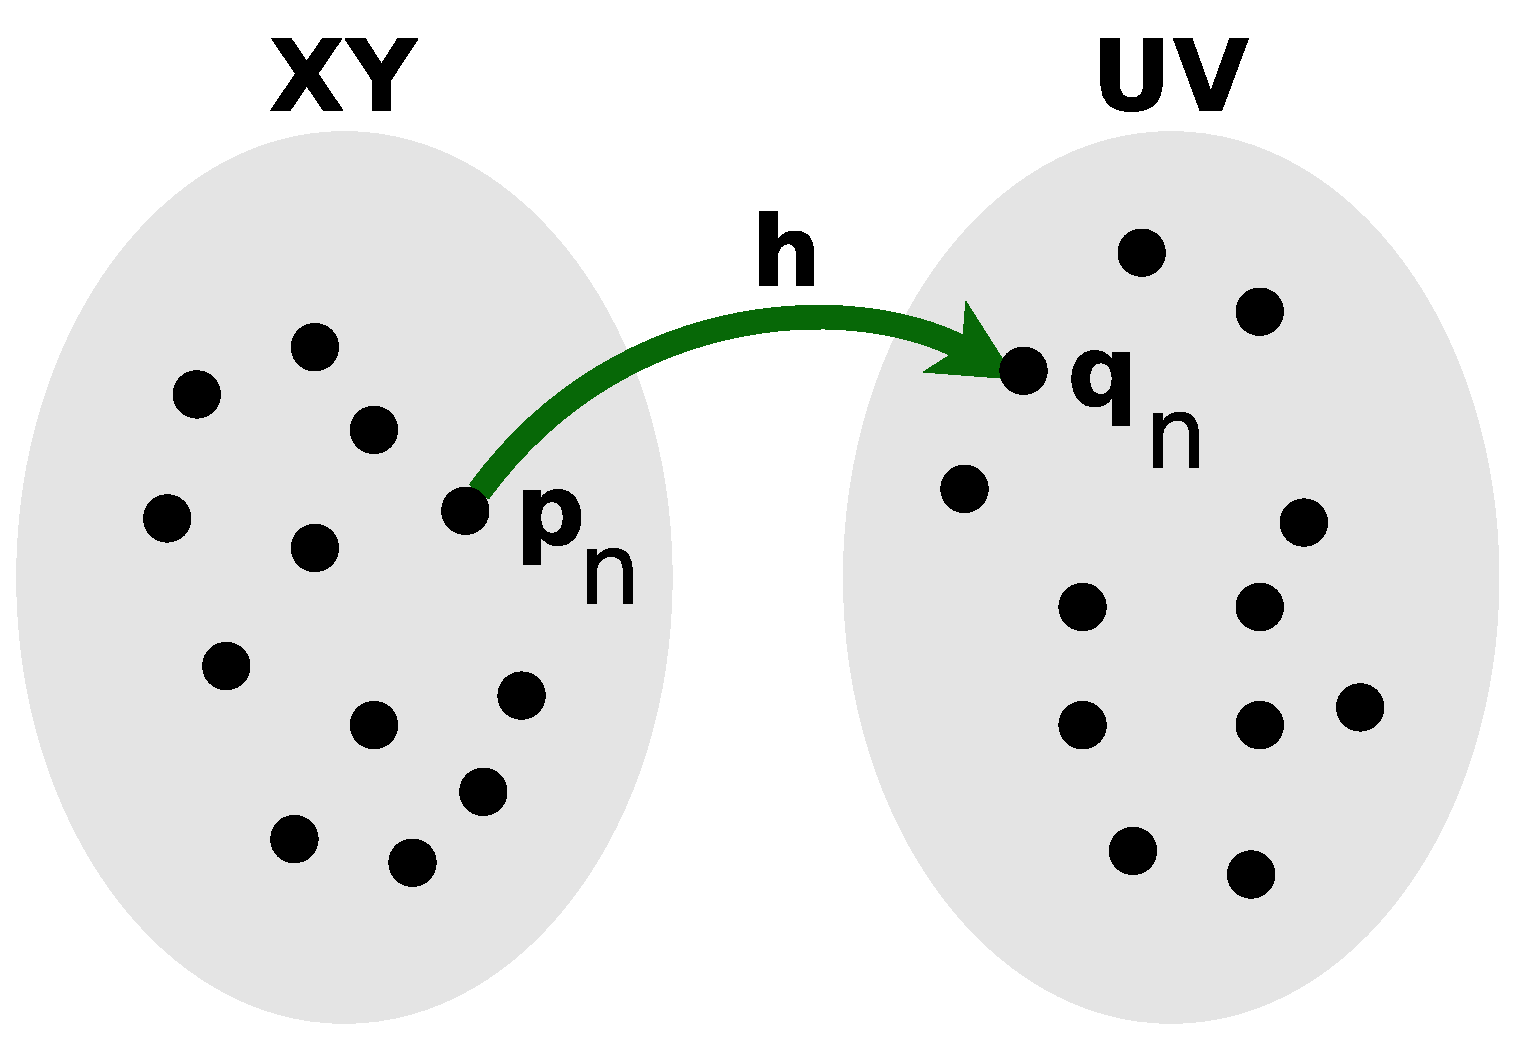
\includegraphics[width=0.8\linewidth]{chapters/inverso-mapeamento/mapeamento.eps} 
\end{minipage}
\begin{minipage}{0.6\textwidth}
\quad Se temos, $N$ pontos (amostras) $\VECTOR{p}_n=[x_n~~y_n]^T\equiv (x_n,y_n)$ no plano $XY \in \mathbb{R}^2$, e
seus correspondentes $\VECTOR{q}_n=[u_n~~v_n]^T\equiv (u_n,y_n)$
no plano $UV \in \mathbb{R}^2$ ,
$\forall n\in \{0, 1, 2, ..., N-1\}$, 
vinculados mediante a função $\VECTOR{h}(x,y): \mathbb{R}^2 \rightarrow \mathbb{R}^2$, 
que é um vetor função de transformação de coordenadas,
$\VECTOR{q}=\VECTOR{h}(\VECTOR{p})$, 
para um ponto $\VECTOR{p} \in XY$ qualquer e seu correspondente $\VECTOR{q} \in UV$.\\
\end{minipage}

Então, podemos modelar  
$[u~~v]^T = \VECTOR{h}(\VECTOR{p})\equiv \VECTOR{h}(x,y)\equiv [h_1(x,y)~~h_2(x,y) ]^T$, 
onde as funções $h_1(x,y)$ e $h_2(x,y)$ $: \mathbb{R}^2 \rightarrow \mathbb{R}$,
são polinômios\footnote{Os polinômios $h_1(x,y)$ e $h_2(x,y)$ são semelhantes, só a notação na escrita foi diferente.} de grau $M$,
\begin{equation}\label{eq:mapeamento:2}
\begin{matrix}
h_1(x,y) & = & +c_{0}\\
              ~ & ~ & +c_{1}~x + c_{2}~y\\
              ~ & ~ & +c_{3}~x^2 +c_{4}~xy + c_{5}~y^2\\
              ~ & ~ &  ...\\
              ~ & ~ & +\sum \limits_{l=0}^{M}c_{\left\{ \frac{M(M+1)}{2}+l\right\}}~x^{M-l}y^{l};
\end{matrix} 
\qquad
\begin{matrix}
h_2(x,y) & = & \sum \limits_{m=0}^{M} \sum \limits_{l=0}^{m}d_{\left\{ \frac{m(m+1)}{2}+l\right\}}~x^{m-l}y^{l}.
       ~ & ~ & ~\\
       ~ & ~ & ~\\
       ~ & ~ & ~\\
       ~ & ~ & ~\\
       ~ & ~ & ~
\end{matrix}
\end{equation}

Assim, o problema de conhecer $\VECTOR{h}(x,y)$ é equivalente ao 
problema de achar os vetores 
$\VECTOR{c}=[c_0~c_1~c_2~...~c_{\left\{ \frac{M(M+3)}{2}\right\}} ]^T$ e
$\VECTOR{d}=[d_0~d_1~d_2~...~d_{\left\{ \frac{M(M+3)}{2}\right\}} ]^T$;
com este fim são usadas as $N$ amostras $\VECTOR{p}_n$ e $\VECTOR{q}_n$,
para  procurar quais são os valores de $\VECTOR{c}$ e $\VECTOR{d}$
que provocam o mínimo erro nos escalares, 
$e_1(\VECTOR{c})$  e $e_2(\VECTOR{d})$.% $:\mathbb{R}^{\left\{ \frac{(M+2)(M+1)}{2}\right\}} \rightarrow \mathbb{R}$.
\begin{equation}\label{eq:mapeamento:3}
 e_1(\VECTOR{c})=||\MATRIX{A}\VECTOR{c}-\VECTOR{u}||^2 \qquad\qquad\qquad  e_2(\VECTOR{d})=||\MATRIX{A}\VECTOR{d}-\VECTOR{v}||^2,
\end{equation}
onde 
\begin{equation}\label{eq:mapeamento:4}
\VECTOR{u}=
\begin{bmatrix}
u_0 \\
u_1 \\
u_2 \\
\vdots \\
u_{N-1}
\end{bmatrix},
\qquad
\VECTOR{v}=
\begin{bmatrix}
v_0 \\
v_1 \\
v_2 \\
\vdots \\
v_{N-1}
\end{bmatrix},
\qquad
\MATRIX{A}=
\begin{bmatrix}
\VECTOR{a}_{00}     & \VECTOR{a}_{01}     & \dots  & \VECTOR{a}_{0(M-1)} \\
\VECTOR{a}_{10}     & \VECTOR{a}_{11}     & \dots  & \VECTOR{a}_{1(M-1)} \\
\VECTOR{a}_{20}     & \VECTOR{a}_{21}     & \dots  & \VECTOR{a}_{2(M-1)} \\
\vdots              & \vdots              & \ddots & \vdots \\
\VECTOR{a}_{(N-1)0} & \VECTOR{a}_{(N-1)1} & \dots  & \VECTOR{a}_{(N-1)(M-1)}
\end{bmatrix}
\end{equation}
\begin{equation}\label{eq:mapeamento:5}
\VECTOR{a}_{nm}=
\begin{bmatrix}
x^m_n  & x^{m-1}_n y_n  & x^{m-2}_n y^2_n    & \dots  & x^{1}_n y^{m-1}_n &  y^m_n 
\end{bmatrix}.
\end{equation}
Um caso especial é quando $\VECTOR{a}_{n0}=1$.
Assim, utilizando o Teorema \ref{theo:minAxbCAxb},
podemos achar o valor $\VECTOR{\hat{c}}$ e $\VECTOR{\hat{d}}$,
que minimizam as funções  $e_1(\VECTOR{\hat{c}})$  e $e_2(\VECTOR{\hat{d}})$:
\begin{equation}\label{eq:mapeamento:6}
\VECTOR{\hat{c}}=
\left[ \MATRIX{A}^{\transpose}  \MATRIX{A} \right]^{-1}\MATRIX{A}^{\transpose} \VECTOR{u},
\qquad \qquad \qquad \qquad
\VECTOR{\hat{d}}=
\left[ \MATRIX{A}^{\transpose}  \MATRIX{A} \right]^{-1}\MATRIX{A}^{\transpose} \VECTOR{v}.
\end{equation}

Devemos ter cuidado, para que exista uma solução única para $\VECTOR{\hat{c}}$ e $\VECTOR{\hat{d}}$,
que o número de linhas de $\MATRIX{A}$ deve ser maior ou igual ao número de suas colunas\footnote{ Que
é equivalente ao número de elementos de $\VECTOR{\hat{c}}$ e $\VECTOR{\hat{d}}$}.
Assim, devemos escolher um valor $M$ que cumpra a seguinte relação com $N$,
\begin{equation}\label{eq:mapeamento:5}
N\geq \frac{(M+1)(M+2)}{2}.
\end{equation}
\end{theorem}


